\section{Motivation}
\label{sec:motivation}
Die Forschung im Bereich der Robotik ist ein immer weiter fortschreitender Prozess. Eine besondere Domäne innerhalb dessen ist die autonome Navigation sowie Steuerung von unbemannten Flugsystemen. Dies findet Anwendung in der Erkundung von unbekannten oder gefahrenträchtigen Gebieten. Dabei müssen nicht nur die physikalischen Eigenschaften der Drohne betrachtet werden sondern auch die Fusion verschiedenster Sensoren.\\

\noindent
Ein wichtiges Kriterium in der Entwicklung autonomer Roboter ist die Erkennung von Hindernissen in Echtzeit. Dabei muss jedoch zuerst definiert werden was vom System als potentielles Hindernis erkannt werden soll. Einerseits sind alle Objekte welche sich in der unmittelbaren Nähe des Systems befinden eine Gefahrenquelle, andererseits wird im Falle Kamera basierter Navigation von einer Bewegung in Blickrichtung ausgegangen. Dies schließt Objekte welche sich außerhalb des Sichtfeldes, also neben oder hinter der Kamera befinden, für die Erfassung durch die Algorithmen aus. Auch sehr weit entfernte Objekte sind prinzipiell nicht als Hindernis anzusehen, wobei sich die maximale Gefahrendistanz relativ zur aktuellen Geschwindigkeit verhält. Unter Betrachtung dieser Gesichtspunkte wird ein Hindernis innerhalb dieser Arbeit als ein Objekt definiert welches sich innerhalb eines definierten Distanzbereichs und innerhalb des Sichtfeldes der Kamera befindet.\\

\noindent
Die hauptsächliche Anwendung des im Rahmen dieser Arbeit entwickelten Systems zielt auf die autonome Navigation von Unbemannten Flugsystemen ab. Weitere Anwendungsbereiche können sowohl komplexerer als auch einfacherer Natur sein. Prinzipiell ist es möglich die entwickelten Algorithmen im Automobil Bereich zu verwenden um beispielsweise Objekte vor oder Hinter dem Kraftfahrzeug zu erkennen und die Distanz zu berechnen. Weiterhin ist es vorstellbar grobe kartographische Höhen Klassifikationen vorzunehmen, um Bild basiert eine Höhenkarte geographischer Areale zu erstellen. Das jeweilige Anwendungsszenario richtet sich jedoch dabei nach der verwendeten Hardware. 

\section{Setup}
\label{sec:setup}

Die aktive Entwicklung der Algorithmen erfolgte im Hinblick auf eine Verwendun dieser durch das von Ascending Technologies \cite{asctec} entwickeltes UAS (Unmanned Aerial System) Pelican (Abbildung \ref{img:pelican}).
Es handelt sich dabei um einen Quattrocopter welcher für den Forschungsbereich entwickelt wurde. Dieser ist mit einem Bordcomputer ausgestattet welche die nötige Leistung für die Entwicklung der Algorithmen bereitstellt (3rd Generation Intel Core i7). Weiterhin wurden zwei MatrixVision BlueFOX mv-MLC200wC Industriekameras \cite{matrixvision} als visuelles System verwendet. Die maximale Auflösung beider Kameras beträgt $752\times480$ bei 60 möglichen Bildern pro Sekunde, in Abhängigkeit verschiedener Parameter (verwendetet Verschlusszeit, aufgenommene Bitrate, u.a). Für den Echtzeit Aspekt des Systems werden beide Kameras im horizontalen und vertikalen Binning verwendet. Dies reduziert die Anzahl der Bildpunkte in beiden Dimensionen auf $376\times240$, wodurch der Berechnungsaufwand verringert und die die Aufnahmerate der Kameras auf bis zu 170 Einzelbilder pro Sekunde maximiert wird.
\noindent
Für die Entwicklung der Algorithmen wurde die freie Computer Vision Bibliothek OpenCV \cite{opencv} verwendet. Diese stellt benötigte algebraische Grundoperationen, sowie bestimmte Algorithmen welche im Rahmen dieser Arbeit genutzt wurden, zur Verfügung.
	% TODO Setup erweitern --> mehr?!
\begin{figure}[h]
	\centering
	\begin{tabular}{cc}
	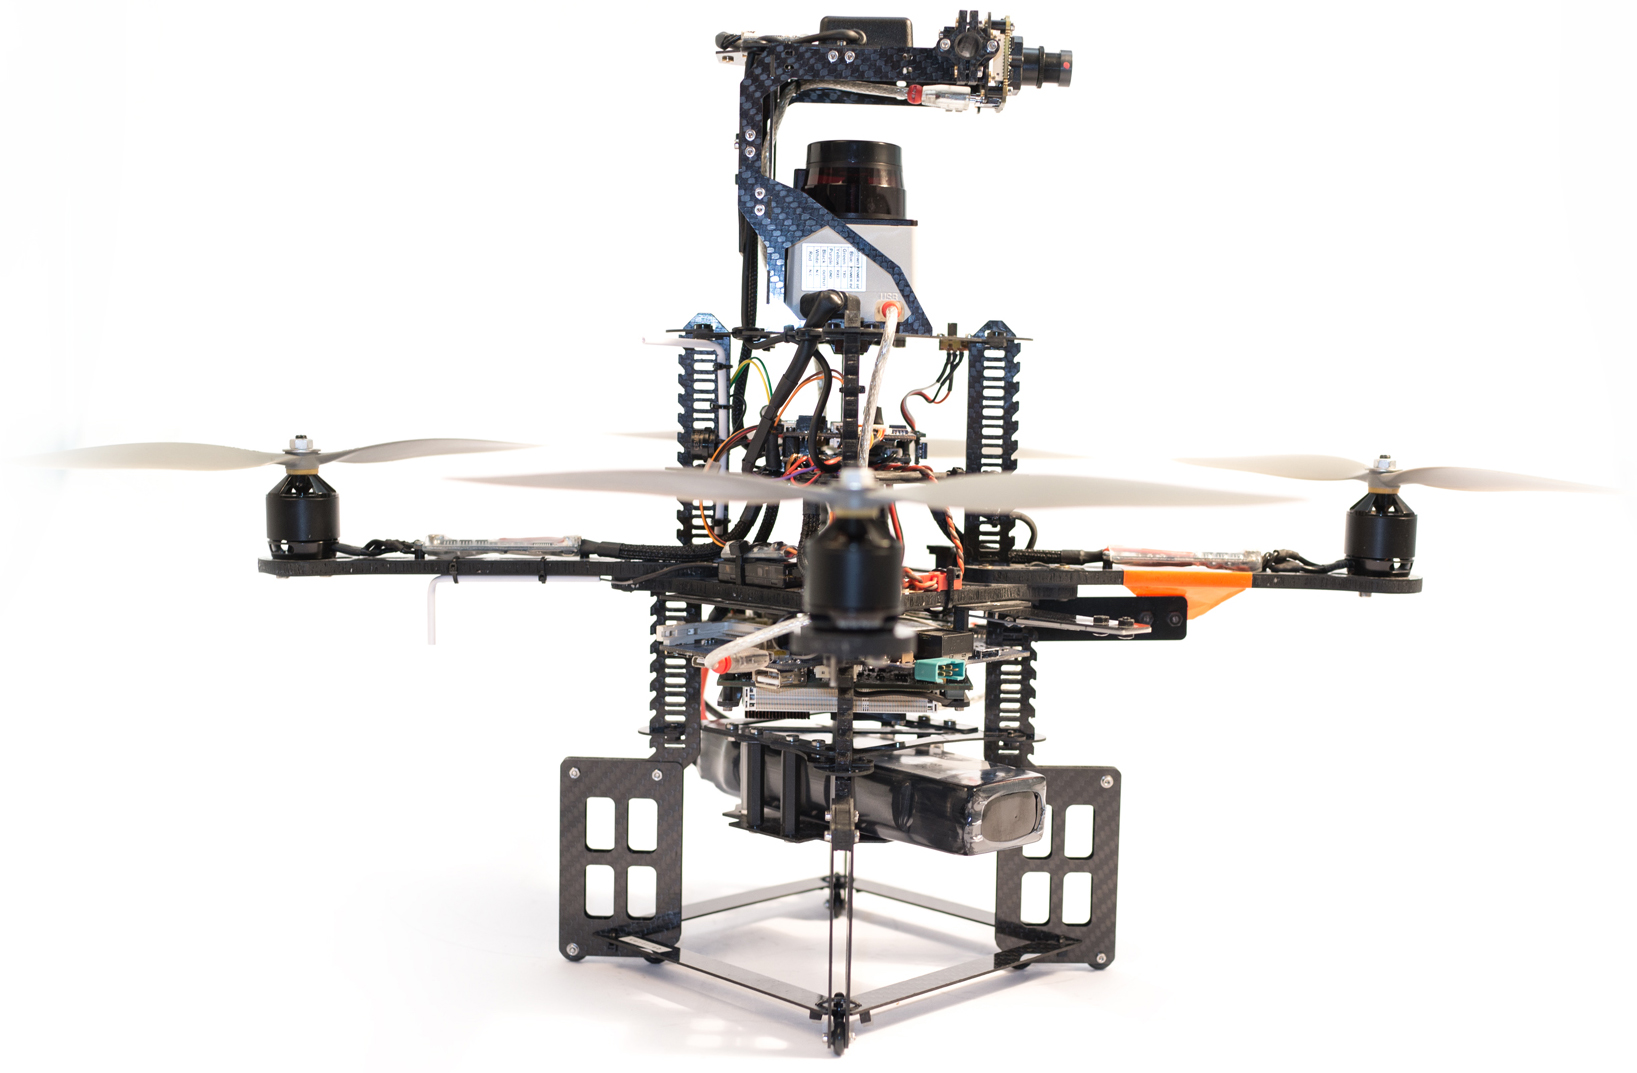
\includegraphics[width=6cm]{img/pelican} &
	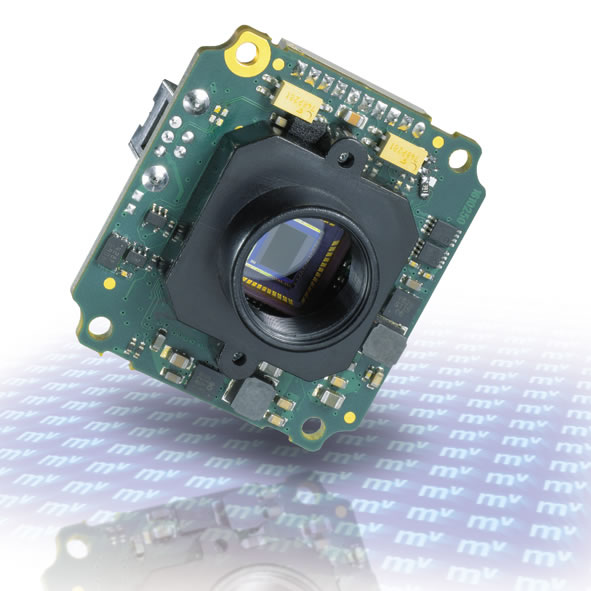
\includegraphics[width=6cm]{img/camera}
	\end{tabular}
	\caption{AscTec Pelika (links), MatrixVision BlueFOX mv-MLC200wC (rechts)}
	\label{img:pelican}
\end{figure}


\section{Ziel der Arbeit}
\label{sec:ziel_der_arbeit}
Mithilfe photogrammetrischer Verfahren ist es mögliche räumliche Tiefe aus zweidimensionalen Daten zu berechnen. Dabei gilt die Verwendung Stereobild basierter Daten als ein einfachste Möglichkeit Disparitäten zwischen korrespondierenden Pixeln zu bestimmen um damit einen räumlichen Eindruck der abgebildeten Szenerie zu erhalten. \\
%Unter Betrachtung dieser Techniken wurde im Rahmen dieser Arbeit \\

\noindent
Vor diesem Hintergrund werden zunächst einige State of the Art Algorithmen beschrieben wobei dabei zwischen aktiven und passiven optischen Systemen unterschieden wird. Diese Einteilung dient einerseits dafür einen Überblick über bereits bestehende Techniken sowie implementierte System zu erhalten, andererseits um auch die Vor und Nachteile der jeweiligen Technik herauszuarbeiten. Kapitel \ref{chp:concepts} beleuchtet zugrundeliegende Konzepte und Algorithmen, dabei liegt der Fokus primär auf essenziell notwendigen Techniken für die im Rahmen dieser Arbeit entwickelten Systeme. Des Weiteren wird das genutzte Framework sowie dessen Funktionsweise erläutert. Im Anschluss daran beschreibt Kapitel \ref{chp:developed_algorithms} die beiden entwickelten Algorithmen zur Hinderniserkennung detailliert. Anschließend daran erfolgt die Evaluation beider Systeme unter den Gesichtspunkten der Robustheit sowie der Performance jedes einzelnen Algorithmus. Weitere Tests zur zukünftigen Verbesserung der Algorithmen weisen auf welches aktuellen Limitierungen durch einerseits genutzte Konzepte vorliegen. Kapitel \ref{chp:conflicts} erläutert eben diese Limitierungen und gibt Ansätze zur Lösung aus der Fachliteratur sowie eigene Konzepte zur Bewältigung dieser. Die anschliessende Diskussion wertet die im Rahmen der Evaluation in Kapitel \ref{chp:evaluation} erlangten Ergebnisse weitergehend aus und stellt beide Algorithmen aktiv gegenüber. Kapitel \ref{chp:fazit} zieht ein Ré­su­mé aus den Ergebnissen der Arbeit und gibt einen Ausblick auf mögliche zukünftige Arbeiten in diesem Bereich.